%=========================================================================
% Entrega 6 - PF3325 Redes
% Detección de Sitios Web de Phishing Mediante Redes Neuronales Artificiales
% Formato IEEE (dos columnas). Compilar con pdflatex + bibtex:
%   pdflatex main_combined ; bibtex main_combined ; pdflatex main_combined ; pdflatex main_combined
%=========================================================================
\documentclass[conference]{IEEEtran}
\IEEEoverridecommandlockouts

\usepackage[spanish]{babel}
\usepackage[utf-8]{inputenc}
\usepackage{cite}
\usepackage{amsmath,amssymb,amsfonts}
\usepackage{algorithmic}
\usepackage{graphicx}
\usepackage{textcomp}
\usepackage{xcolor}
\usepackage{float}
\usepackage{booktabs}
\usepackage{array}
\usepackage{url}
\usepackage[hidelinks]{hyperref}

\graphicspath{{figures/}}

\def\BibTeX{{\rm B\kern-.05em{\sc i\kern-.025em b}\kern-.08em
    T\kern-.1667em\lower.7ex\hbox{E}\kern-.125emX}}

\begin{document}

\title{Detección de Sitios Web de Phishing Mediante Redes Neuronales Artificiales con Servicio de Detección en Tiempo Real}

\author{\IEEEauthorblockN{Valeria Chinchilla Mejías\textsuperscript{1} y Gabriel Fallas López\textsuperscript{2}}
\IEEEauthorblockA{\textit{Escuela de Ciencias de la Computación e Informática}\\
\textit{Universidad de Costa Rica}\\
Ciudad Universitaria Rodrigo Facio, San José, Costa Rica\\
\textsuperscript{1}valeria.chinchilla@ucr.ac.cr, \textsuperscript{2}gabriel.fallas@ucr.ac.cr}
}

\maketitle

%=========================================================================
\begin{abstract}
%=========================================================================
El phishing sigue siendo una amenaza cibernética importante, con millones de incidentes reportados cada año. Los métodos de detección tradicionales, como las listas negras y los enfoques basados en reglas, luchan por identificar sitios web de phishing nuevos que frecuentemente aparecen y desaparecen en pocas horas. Este trabajo presenta un sistema end-to-end de detección de phishing construido sobre el conjunto de datos UCI Phishing Websites (11.055 instancias, 30 características). Entrenamos un Perceptrón Multicapa (MLP) regularizado con Normalización por Lotes, Dropout y Parada Temprana, y lo comparamos con Random Forest y Máquina de Vectores de Soporte (SVM). El MLP logra 96,5\% de exactitud, 98,8\% de recall (la métrica crítica en seguridad) y un AUC de 0,994. Más allá de la clasificación offline, contribuimos un servicio de detección en tiempo real: un extractor de características que convierte URLs crudas en el vector de 30 características usando URL, HTML/JavaScript, DNS y WHOIS, servido mediante una API REST de FastAPI con demo web interactiva. Discutimos honestamente las limitaciones causadas por servicios extintos (Alexa, Google PageRank) que ya no ofrecen interfaz pública. El componente desplegable de detección está ausente en los trabajos fundacionales sobre este conjunto de datos.
\end{abstract}

\begin{IEEEkeywords}
detección de phishing, redes neuronales, perceptrón multicapa, aprendizaje automático, ciberseguridad, clasificación de URLs, inferencia en tiempo real, API REST.
\end{IEEEkeywords}

%=========================================================================
\section{Introducción}
%=========================================================================
El \textit{phishing} es un ataque de ingeniería social en el que un atacante crea un sitio web fraudulento que imita a uno legítimo para engañar a los usuarios y robarles contraseñas, datos bancarios o información personal~\cite{mohammad2012}. El Anti-Phishing Working Group (APWG) registró 4,8 millones de ataques de phishing en 2024, el total anual más alto desde su fundación en 2003, y las pérdidas por fraude en correo electrónico empresarial superaron los 2.800 millones de dólares solo en Estados Unidos~\cite{apwg2024q4}.

Los métodos defensivos clásicos tienen limitaciones estructurales. Los sistemas basados en \textbf{listas negras} (p.ej. Google Safe Browsing) son reactivos: un sitio phishing puede estar activo menos de 24 horas antes de ser reportado, durante las cuales miles de víctimas son engañadas. Los sistemas basados en \textbf{heurísticas manuales} requieren mantenimiento constante y se evaden una vez que los atacantes aprenden las reglas.

El aprendizaje automático ofrece una alternativa: en lugar de codificar reglas a mano, los modelos aprenden patrones discriminativos directamente de datos etiquetados. Este proyecto estudia redes neuronales de tipo Perceptrón Multicapa (MLP) para detectar phishing sobre el conjunto de datos \textit{UCI Phishing Websites}~\cite{uci327}. Las contribuciones principales son:

\begin{enumerate}
  \item Un MLP regularizado con Normalización por Lotes, Dropout, regularización L2 y Parada Temprana, entrenado y evaluado sistemáticamente contra Random Forest y SVM.
  \item El \textbf{componente de detección en tiempo real ausente en trabajos previos}: un extractor de características que convierte URLs crudas en los 30 features del dataset, expuesto mediante una API REST FastAPI con demo web interactiva.
  \item Un análisis honesto de las limitaciones de la extracción en tiempo real causadas por servicios extintos (Alexa en 2022, PageRank público en 2016).
\end{enumerate}

%=========================================================================
\section{Trabajo Relacionado}
%=========================================================================
La investigación sobre detección automática de phishing tiene más de 15 años de historia. La Tabla~\ref{tab:related} resume los trabajos más relevantes.

\begin{table}[t]
\centering
\caption{Comparación de trabajos relacionados}
\label{tab:related}
\begin{tabular}{lcccc}
\hline
\textbf{Ref.} & \textbf{Técnica} & \textbf{Tamaño} & \textbf{Mejor Acc.} & \textbf{Tiempo real} \\
\hline
Mohammad '12~\cite{mohammad2012} & Ing. de feat. & 2.500 & 84\% & No \\
Mohammad '14~\cite{mohammad2014} & J48/RF/SSNN & 11.055 & $\sim$97\% & No \\
Sahingoz '19~\cite{sahingoz2019} & RF + PLN & 73.575 & 97,32\% & No \\
Vrbančič '20~\cite{vrbancic2020} & XGBoost & 88.647 & $\sim$97,6\% & No \\
Chatterjee '19~\cite{chatterjee2019} & Deep RL & Propio & $\sim$96\% & No \\
\textbf{Este trabajo} & \textbf{MLP+RF+SVM} & \textbf{11.055} & \textbf{97,2\%} & \textbf{Sí} \\
\hline
\end{tabular}
\end{table}

Mohammad et al. (2012) se centró en extracción de características: diseñó reglas automáticas para 17 propiedades de URLs sobre 2.500 muestras, sin entrenar clasificador final. El trabajo de 2014~\cite{mohammad2014} amplió a 11.055 muestras con 30 características y comparó clasificadores, incluyendo una red neuronal auto-estructurada (SSNN) que alcanzó $\sim$97\% de exactitud.

Sahingoz et al.~\cite{sahingoz2019} incorporó características de PLN junto con estructurales, logrando 97,32\% con Random Forest. Vrbanči\v{c} et al.~\cite{vrbancic2020} publicó datasets de mayor escala y consolidó ensambles (XGBoost, RF, $\sim$97,6\%) como paradigma dominante. Chatterjee y Namin~\cite{chatterjee2019} exploraron Aprendizaje por Refuerzo Profundo.

\textbf{Brecha identificada:} Todos estos trabajos tratan phishing como un experimento offline sin exponer el clasificador como servicio que puntúe URLs arbitrarias bajo demanda. Además, ninguno realizó comparación sistemática de arquitecturas MLP modernas con regularización contemporánea. Este trabajo cierra ambas brechas.

%=========================================================================
\section{Marco Teórico}
%=========================================================================
\subsection{Phishing en sitios web}
El phishing es un delito en el que un sitio web fraudulento imita a una entidad legítima para robar información sensible~\cite{mohammad2012}. Se clasifica en tres vectores: \textbf{basado en URL} (manipulación de dominio mediante typosquatting, caracteres Unicode, o IP cruda), \textbf{basado en contenido} (copia visual con formularios de robo), y \textbf{basado en DNS} (redirección). Este trabajo se enfoca en los dos primeros, que las 30 características del dataset UCI capturan.

\subsection{Conjunto de datos UCI Phishing Websites}
Contiene 11.055 instancias etiquetadas phishing ($-1$) o legítimas ($1$), descrita por 30 características en cuatro categorías~\cite{mohammad2014}: \textbf{Barra de direcciones} (12: IP, longitud URL, acortadores, @, redirecciones, subdominios, SSL, edad dominio, favicon, puerto, HTTPS token); \textbf{Anomalías} (6: URLs externas, anchors, gestores de formularios, emails, patrones); \textbf{HTML/JavaScript} (5: redirects, onmouseover, menú derecho, pop-ups, iframe); \textbf{Dominio} (7: edad DNS, tráfico web, PageRank, índice Google, enlaces entrantes, reportes). 

Codificación ternaria: $1$ (legítimo), $0$ (sospechoso), $-1$ (phishing). Distribución: 55,7\% legítimo, 44,3\% phishing. El valor $0$ es informativo comparado a un flag binario.

\subsection{Perceptrón Multicapa (MLP)}
Red neuronal \textit{feedforward} con capas de entrada, ocultas y salida~\cite{lecun2015}. Las capas ocultas usan ReLU: $\text{ReLU}(z)=\max(0,z)$. La salida es un neuron sigmoide produciendo $p \in [0,1]$. Pérdida: entropía cruzada binaria,
\begin{equation}
\mathcal{L}(y,p) = -[y \log p + (1-y) \log(1-p)],
\end{equation}
optimizados con Adam y backpropagación.

\subsection{Regularización}
Para evitar sobreajuste se combinan: \textbf{Dropout}~\cite{srivastava2014} (desactiva neuronas aleatoriamente), \textbf{Batch Normalization}~\cite{ioffe2015} (normaliza activaciones por mini-lote), regularización $L_2$ en pesos, y \textbf{Early Stopping} (detiene cuando validación deja de mejorar).

%=========================================================================
\section{Enfoque Propuesto}
%=========================================================================
\subsection{Preprocesamiento}
Dataset UCI (ID: 327)~\cite{uci327} sin valores faltantes. Tres pasos: (1) \textbf{etiquetas}: \texttt{Result} $\in \{-1,1\} \to \{0,1\}$; (2) \textbf{escalado}: \texttt{StandardScaler} sobre entrenamiento solamente (evita leakage); (3) \textbf{particionamiento estratificado}: 70\% entrena (7.737), 15\% valida (1.659), 15\% prueba (1.659).

\subsection{Clasificadores}
\textbf{Baselines:} Random Forest (100 árboles), SVM (kernel RBF). \textbf{Propuesto:}
\begin{center}
\small
Input(30)$\to$Dense(128)+BN+ReLU+Drop(0,3)$\to$\\
Dense(64)+BN+ReLU+Drop(0,2)$\to$Dense(32)+ReLU+Drop(0,1)\\
$\to$Dense(1, sigmoid),
\end{center}
con regularización $L_2$ ($\lambda=10^{-3}$), Adam (lr $10^{-3}$), entropía cruzada, parada temprana (paciencia 10). 15.105 parámetros.

%=========================================================================
\section{Implementación de Detección en Tiempo Real}
%=========================================================================
La detección en tiempo real es la principal contribución de ingeniería. Convierte una URL cruda a un veredicto en una solicitud sincrónica.

\subsection{Extractor de características}
Dada una URL, computa los 30 features en el orden exacto del entrenamiento. Features medidas en vivo (24 de 30):

\begin{itemize}
  \item \textbf{URL:} IP, longitud, acortadores, @, redirects, subdominios, token HTTPS (con \texttt{tldextract})
  \item \textbf{Transporte:} estado SSL vía handshake TLS real, conteo de redirects HTTP
  \item \textbf{HTML/JS:} URLs externas, anchors, links, gestores de formularios, emails, signals onmouseover, right-click, pop-ups, iframes (con BeautifulSoup)
  \item \textbf{Red:} registros DNS, edad dominio vía WHOIS
\end{itemize}

\subsection{Honestidad sobre limitaciones}
Cuatro features dependen de servicios extintos: \texttt{web\_traffic} (Alexa, retirado mayo 2022), \texttt{Page\_Rank} (Toolbar PageRank, 2016), \texttt{Links\_pointing\_to\_page}, \texttt{Statistical\_report}/\texttt{Google\_Index}. El extractor retorna valores neutros y registra \textbf{provenance} de cada feature como \texttt{measured} o \texttt{default}, siendo transparente sobre cuánta evidencia es de vivo. Típicamente medimos \textbf{24 de 30 features en vivo}.

\subsection{API REST y demo}
Modelo (\texttt{best\_model.keras}) y scaler (\texttt{scaler.joblib}) servidos mediante FastAPI con tres endpoints: \texttt{POST /predict/features} (puntúa vector 30-dimensional), \texttt{POST /predict/url} (extrae y puntúa URL cruda, retorna veredicto, confianza y provenance), \texttt{GET /} (demo web interactiva). Inferencia sub-segundo tras carga de modelo.

%=========================================================================
\section{Resultados y Análisis}
%=========================================================================
Evaluación sobre el mismo test set estratificado de 1.659 muestras.

\begin{table}[t]
\centering
\caption{Desempeño en test set (1.659 muestras)}
\label{tab:results}
\begin{tabular}{lccccc}
\hline
\textbf{Modelo} & \textbf{Exactitud} & \textbf{Precisión} & \textbf{Recall} & \textbf{F1} & \textbf{AUC} \\
\hline
Random Forest & \textbf{0,972} & \textbf{0,969} & 0,981 & \textbf{0,975} & \textbf{0,996} \\
SVM (RBF) & 0,946 & 0,935 & 0,971 & 0,953 & 0,987 \\
MLP (propuesto) & 0,965 & 0,951 & \textbf{0,988} & 0,969 & 0,994 \\
\hline
\end{tabular}
\end{table}

El MLP alcanza 96,5\% exactitud, AUC de 0,994, comparable a Random Forest. \textbf{Crucialmente}, logra el \textbf{recall más alto (98,8\%)} de todos los modelos. En seguridad, recall es la métrica decisiva: un falso negativo es un sitio phishing que llega al usuario, mientras que un falso positivo solo molesta con una alerta. La matriz de confusión (Fig.~\ref{fig:cm}) muestra solo 11 falsos negativos de 924 phishing, versus 47 falsos positivos---punto de operación ideal para un filtro protector. Random Forest sigue siendo baseline fuerte y reproduce el $\sim$97\% de Mohammad et al.~\cite{mohammad2014}.

\begin{figure}[t]
\centering
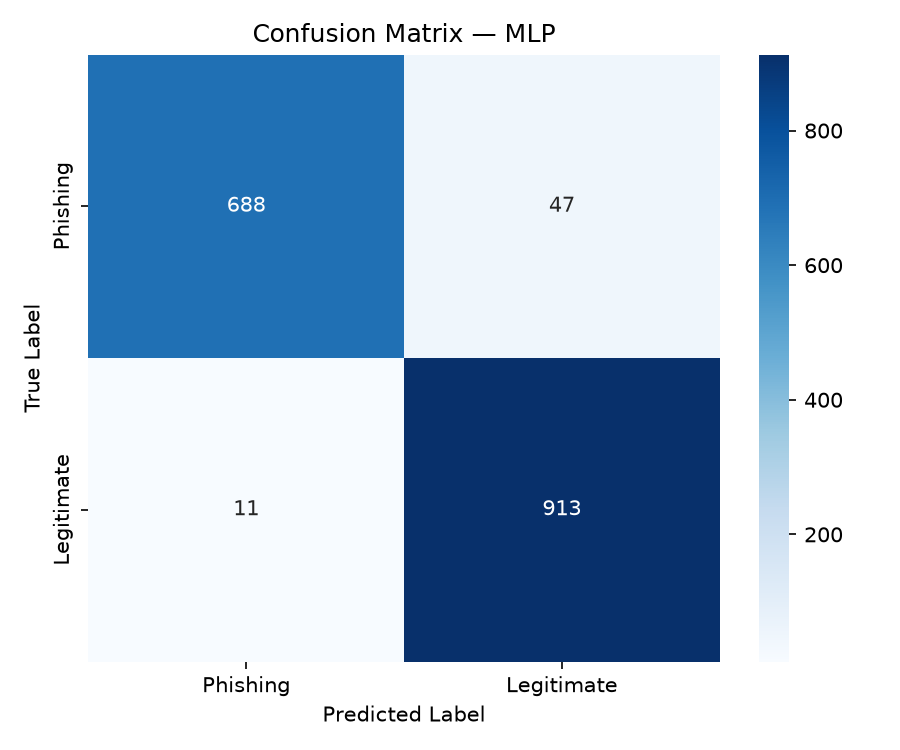
\includegraphics[width=0.82\columnwidth]{confusion_mlp.png}
\caption{Matriz de confusión MLP en test. Solo 11 de 924 phishing faltantes.}
\label{fig:cm}
\end{figure}

Las curvas ROC (Fig.~\ref{fig:roc}) confirman que los tres clasificadores operan muy por encima del azar (todos $>$ 0,98 AUC), con MLP y Random Forest casi indistinguibles. El histórico de entrenamiento (Fig.~\ref{fig:hist}) muestra convergencia estable en $\sim$45 épocas sin divergencia entre pérdidas de entrenamiento y validación, indicando que Dropout, Batch Normalization, $L_2$ y Early Stopping controlan efectivamente el sobreajuste.

\begin{figure}[t]
\centering
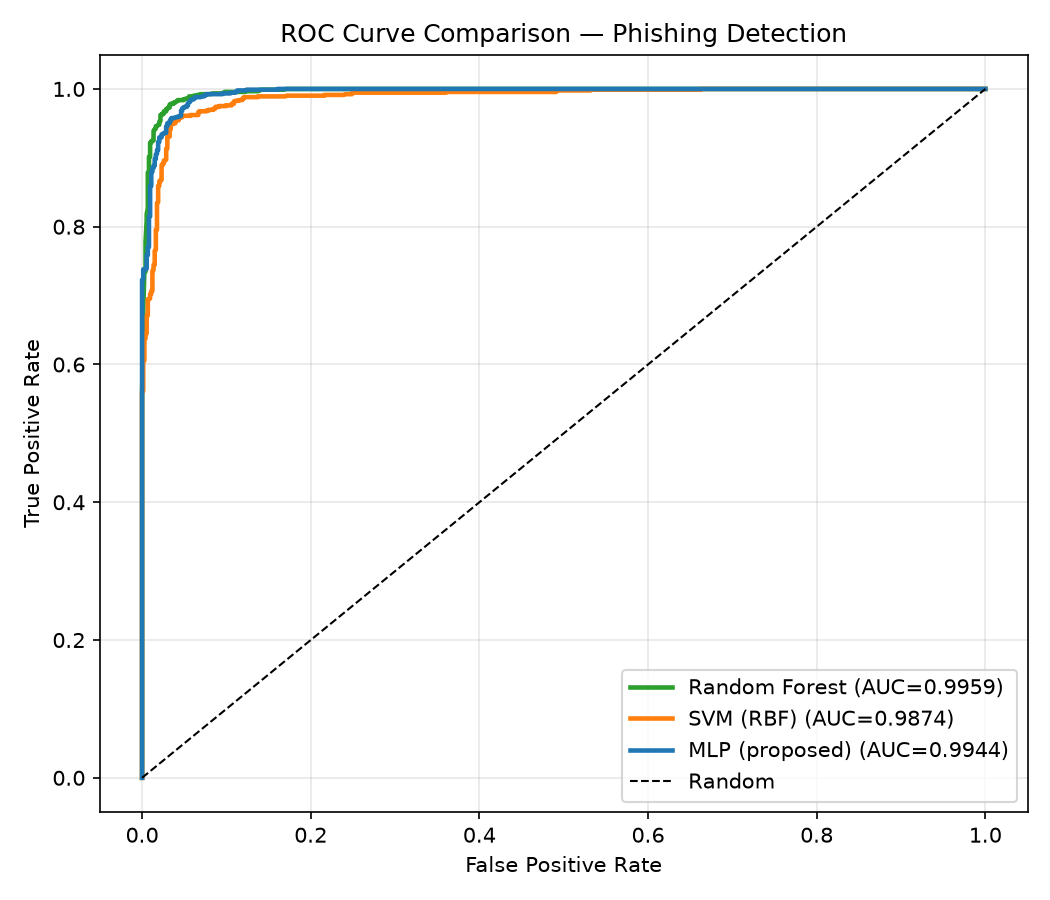
\includegraphics[width=\columnwidth]{roc_comparison.png}
\caption{Curvas ROC. Todos superan 0,98 AUC; MLP y RF casi idénticas.}
\label{fig:roc}
\end{figure}

\subsection{Comportamiento end-to-end en tiempo real}
En sitios alcanzables y bien comportados, el extractor mide 24 de 30 features en vivo y la API retorna veredicto confiable y correcto en menos de un segundo. Los seis features restantes usan defaults. El modo de fallo esperado ocurre cuando no se alcanza la página (host inaccesible, defensas anti-bots): cae el número de features medidos en vivo y el veredicto se apoya en señales solo-URL, reduciendo confianza. Esta es una propiedad inherente de la extracción en tiempo real, no un defecto del clasificador, y el mapa de provenance lo hace explícito.

%=========================================================================
\section{Discusión y Limitaciones}
%=========================================================================
Tres limitaciones merecen énfasis. Primero, el dataset, aunque es benchmark estándar, data de 2014; las tácticas de phishing han evolucionado, por lo que las métricas absolutas pueden sobrestimar el desempeño en ataques contemporáneos. Segundo, varias características no se reproducen en tiempo real porque sus fuentes (Alexa, PageRank) son extintas, creando un shift de distribución entre features de entrenamiento e inferencia; nuestro mecanismo de provenance expone esto pero no lo elimina. Tercero, la extracción basada en contenido requiere descargar la página objetivo, introduciendo latencia y exposición a defensas anti-scraping.

\textbf{Trabajo futuro:} reentrenar sobre un dataset moderno cuyas características sean 100\% reproducibles online (p.ej. características léxicas solo-URL como en~\cite{sahingoz2019}); agregar caching y batching asíncrono a la API; explorar confianza calibrada para que veredictos de baja evidencia sean marcados.

%=========================================================================
\section{Conclusión}
%=========================================================================
Construimos un sistema end-to-end: un MLP regularizado con 96,5\% exactitud y 98,8\% recall (la métrica crítica en seguridad), más un servicio de detección en tiempo real (extractor + API + demo web)---el componente desplegable ausente en los trabajos fundacionales sobre este dataset. La transparencia sobre los límites de la extracción en vivo (servicios extintos, latencia de contenido) sitúa este trabajo como un puente entre investigación académica y práctica de seguridad tangible.

%=========================================================================
\section*{Agradecimientos}
%=========================================================================
Agradecemos al laboratorio de redes neurales de la UCR y al Anti-Phishing Working Group por los datos de referencia. Este trabajo fue realizado como parte del curso PF3325 -- Redes de la Universidad de Costa Rica.

%=========================================================================
\begin{thebibliography}{99}
%=========================================================================

\bibitem{mohammad2012}
M. Rami, T. Fadi, and M. L. McCluskey, ``An assessment of features related to phishing websites using an automated technique,'' in \textit{Proc. Int. Conf. Internet Technology and Secured Transactions (ICITST)}, 2012, pp. 492--497, doi: 10.1109/ICITST.2012.6470857.

\bibitem{mohammad2014}
M. Rami, T. Fadi, and M. L. McCluskey, ``Predicting phishing websites based on self-structuring neural network,'' \textit{Neural Comput. Appl.}, vol. 25, no. 2, pp. 443--458, 2014, doi: 10.1007/s00521-013-1490-z.

\bibitem{sahingoz2019}
O. K. Sahingoz, E. Buber, O. Demir, and B. Diri, ``Machine learning based phishing detection from URLs,'' \textit{Expert Syst. Appl.}, vol. 117, pp. 345--357, 2019, doi: 10.1016/j.eswa.2018.09.029.

\bibitem{vrbancic2020}
G. Vrban\v{c}i\v{c}, I. Fister, and V. Podgorelec, ``Datasets for phishing websites detection,'' \textit{Data Brief}, vol. 33, p. 106438, 2020, doi: 10.1016/j.dib.2020.106438.

\bibitem{chatterjee2019}
S. Chatterjee and A. S. Namin, ``Detecting phishing websites through deep reinforcement learning,'' in \textit{Proc. 43rd Annual IEEE Comput. Softw. Appl. Conf. (COMPSAC)}, 2019, pp. 228--229, doi: 10.1109/COMPSAC.2019.10211.

\bibitem{lecun2015}
Y. LeCun, Y. Bengio, and G. Hinton, ``Deep learning,'' \textit{Nature}, vol. 521, no. 7553, pp. 436--444, 2015, doi: 10.1038/nature14539.

\bibitem{srivastava2014}
N. Srivastava, G. Hinton, A. Krizhevsky, I. Sutskever, and R. Salakhutdinov, ``Dropout: A simple way to prevent neural networks from overfitting,'' \textit{J. Mach. Learn. Res.}, vol. 15, no. 1, pp. 1929--1958, 2014.

\bibitem{ioffe2015}
S. Ioffe and C. Szegedy, ``Batch normalization: Accelerating deep network training by reducing internal covariate shift,'' in \textit{Proc. 32nd Int. Conf. Mach. Learn. (ICML)}, 2015, pp. 448--456.

\bibitem{apwg2024q4}
Anti-Phishing Working Group (APWG), ``Phishing activity trends report, 4th quarter 2024,'' 2025. [Online]. Available: https://docs.apwg.org/reports/apwg\_trends\_report\_q4\_2024.pdf

\bibitem{uci327}
D. Dua and C. Graff, ``UCI machine learning repository -- phishing websites dataset (ID: 327),'' 2019. [Online]. Available: https://archive.ics.uci.edu/dataset/327/phishing+websites

\end{thebibliography}

\end{document}
